\section{Análisis técnico-económica}
% FELIX_RUIZ_JAVIER_DISEÑO_ELECTROGONIÓMETRO_MEDIR

Siguiendo la metodología VDI 2225 \cite{VDI2225}, se establecen criterios para evaluar los aspectos técnicos y económicos de las soluciones propuestas. La evaluación técnica y económica se presenta en las Tablas \ref{tab:eval_tecnica} y \ref{tab:eval_economica}, respectivamente. Los criterios tienen pesos diferenciados en el cálculo ponderado, reflejando su importancia en el sistema de acuerdo con la siguiente nomenclatura:

\begin{itemize}
	\setlength\itemsep{0em}
	\item El valor de \textbf{g} representa el peso ponderado en función de la importancia del criterio de evaluación.
	\begin{itemize}
		\setlength\itemsep{0em}
		\item 1 = No importante.
		\item 2 = Poco importante.
		\item 3 = Importante.
		\item 4 = Muy importante.
	\end{itemize}
	\item El valor de \textbf{p} representa un puntaje de 0 a 4 (Escala de valores VDI 2225), siendo:
	\begin{itemize}
		\setlength\itemsep{0em}
		\item 0 = No satisface.
		\item 1 = Apenas aceptable.
		\item 2 = Suficiente.
		\item 3 = Bien.
		\item 4 = Excelente (Ideal).
	\end{itemize}
\end{itemize}


\begin{table}[h]
	\centering
	\caption[Evaluación técnica de los conceptos de solución.]{Evaluación técnica de los conceptos de solución. Fuente: Elaboración propia.}
	\resizebox{0.9\textwidth}{!}{
		\begin{tabular}{|c|c|c|c|c|c|c|c|c|c|c|}
			\hline
			\multicolumn{3}{|c|}{\textbf{Evaluación Técnica}} & \multicolumn{2}{c|}{\cellcolor[rgb]{ 1,  0,  0}\textcolor[rgb]{ 1,  1,  1}{\textbf{Solución 1}}} & \multicolumn{2}{c|}{\cellcolor[rgb]{ 0,  0,  1}\textcolor[rgb]{ 1,  1,  1}{\textbf{Solución 2}}} & \multicolumn{2}{c|}{\cellcolor[rgb]{ .298,  .835,  .078}\textbf{Solución 3}} & \multicolumn{2}{c|}{\cellcolor[rgb]{ 1,  .82,  .4}\textbf{Ideal}} \bigstrut\\
			\hline
			\textbf{Nro} & \textbf{Criterio} & \textbf{g} & \textbf{p} & \textbf{p x g} & \textbf{p} & \textbf{p x g} & \textbf{p} & \textbf{p x g} & \textbf{p} & \textbf{p x g} \bigstrut\\
			\hline
			\textbf{1} & \multicolumn{1}{l|}{\textbf{Tamaño}} & \multicolumn{1}{r|}{2} & \multicolumn{1}{r|}{\cellcolor[rgb]{ .949,  .863,  .859}3} & \multicolumn{1}{r|}{6} & \multicolumn{1}{r|}{\cellcolor[rgb]{ .863,  .902,  .945}3} & \multicolumn{1}{r|}{6} & \multicolumn{1}{r|}{\cellcolor[rgb]{ .922,  .945,  .871}2} & \multicolumn{1}{r|}{4} & \multicolumn{1}{r|}{\cellcolor[rgb]{ .992,  .914,  .851}4} & \multicolumn{1}{r|}{8} \bigstrut\\
			\hline
			\textbf{2} & \multicolumn{1}{l|}{\textbf{Dificultad de fabricación}} & \multicolumn{1}{r|}{2} & \multicolumn{1}{r|}{\cellcolor[rgb]{ .949,  .863,  .859}4} & \multicolumn{1}{r|}{8} & \multicolumn{1}{r|}{\cellcolor[rgb]{ .863,  .902,  .945}3} & \multicolumn{1}{r|}{6} & \multicolumn{1}{r|}{\cellcolor[rgb]{ .922,  .945,  .871}2} & \multicolumn{1}{r|}{4} & \multicolumn{1}{r|}{\cellcolor[rgb]{ .992,  .914,  .851}4} & \multicolumn{1}{r|}{8} \bigstrut\\
			\hline
			\textbf{3} & \multicolumn{1}{l|}{\textbf{Calibración}} & \multicolumn{1}{r|}{4} & \multicolumn{1}{r|}{\cellcolor[rgb]{ .949,  .863,  .859}1} & \multicolumn{1}{r|}{4} & \multicolumn{1}{r|}{\cellcolor[rgb]{ .863,  .902,  .945}4} & \multicolumn{1}{r|}{16} & \multicolumn{1}{r|}{\cellcolor[rgb]{ .922,  .945,  .871}2} & \multicolumn{1}{r|}{8} & \multicolumn{1}{r|}{\cellcolor[rgb]{ .992,  .914,  .851}4} & \multicolumn{1}{r|}{16} \bigstrut\\
			\hline
			\textbf{4} & \multicolumn{1}{l|}{\textbf{Tiempo de procesamiento}} & \multicolumn{1}{r|}{4} & \multicolumn{1}{r|}{\cellcolor[rgb]{ .949,  .863,  .859}2} & \multicolumn{1}{r|}{8} & \multicolumn{1}{r|}{\cellcolor[rgb]{ .863,  .902,  .945}4} & \multicolumn{1}{r|}{16} & \multicolumn{1}{r|}{\cellcolor[rgb]{ .922,  .945,  .871}4} & \multicolumn{1}{r|}{16} & \multicolumn{1}{r|}{\cellcolor[rgb]{ .992,  .914,  .851}4} & \multicolumn{1}{r|}{16} \bigstrut\\
			\hline
			\textbf{5} & \multicolumn{1}{l|}{\textbf{Interfaz intuitiva}} & \multicolumn{1}{r|}{3} & \multicolumn{1}{r|}{\cellcolor[rgb]{ .949,  .863,  .859}3} & \multicolumn{1}{r|}{9} & \multicolumn{1}{r|}{\cellcolor[rgb]{ .863,  .902,  .945}4} & \multicolumn{1}{r|}{12} & \multicolumn{1}{r|}{\cellcolor[rgb]{ .922,  .945,  .871}4} & \multicolumn{1}{r|}{12} & \multicolumn{1}{r|}{\cellcolor[rgb]{ .992,  .914,  .851}4} & \multicolumn{1}{r|}{12} \bigstrut\\
			\hline
			\textbf{6} & \multicolumn{1}{l|}{\textbf{Facilidad de manejo }} & \multicolumn{1}{r|}{4} & \multicolumn{1}{r|}{\cellcolor[rgb]{ .949,  .863,  .859}3} & \multicolumn{1}{r|}{12} & \multicolumn{1}{r|}{\cellcolor[rgb]{ .863,  .902,  .945}3} & \multicolumn{1}{r|}{12} & \multicolumn{1}{r|}{\cellcolor[rgb]{ .922,  .945,  .871}3} & \multicolumn{1}{r|}{12} & \multicolumn{1}{r|}{\cellcolor[rgb]{ .992,  .914,  .851}4} & \multicolumn{1}{r|}{16} \bigstrut\\
			\hline
			\textbf{7} & \multicolumn{1}{l|}{\textbf{Seguridad}} & \multicolumn{1}{r|}{4} & \multicolumn{1}{r|}{\cellcolor[rgb]{ .949,  .863,  .859}3} & \multicolumn{1}{r|}{12} & \multicolumn{1}{r|}{\cellcolor[rgb]{ .863,  .902,  .945}3} & \multicolumn{1}{r|}{12} & \multicolumn{1}{r|}{\cellcolor[rgb]{ .922,  .945,  .871}4} & \multicolumn{1}{r|}{16} & \multicolumn{1}{r|}{\cellcolor[rgb]{ .992,  .914,  .851}4} & \multicolumn{1}{r|}{16} \bigstrut\\
			\hline
			\textbf{8} & \multicolumn{1}{l|}{\textbf{Facilidad de mantenimiento}} & \multicolumn{1}{r|}{2} & \multicolumn{1}{r|}{\cellcolor[rgb]{ .949,  .863,  .859}3} & \multicolumn{1}{r|}{6} & \multicolumn{1}{r|}{\cellcolor[rgb]{ .863,  .902,  .945}2} & \multicolumn{1}{r|}{4} & \multicolumn{1}{r|}{\cellcolor[rgb]{ .922,  .945,  .871}3} & \multicolumn{1}{r|}{6} & \multicolumn{1}{r|}{\cellcolor[rgb]{ .992,  .914,  .851}4} & \multicolumn{1}{r|}{8} \bigstrut\\
			\hline
			\textbf{9} & \multicolumn{1}{l|}{\textbf{Capacidad de análisis completo}} & \multicolumn{1}{r|}{4} & \multicolumn{1}{r|}{\cellcolor[rgb]{ .949,  .863,  .859}1} & \multicolumn{1}{r|}{4} & \multicolumn{1}{r|}{\cellcolor[rgb]{ .863,  .902,  .945}3} & \multicolumn{1}{r|}{12} & \multicolumn{1}{r|}{\cellcolor[rgb]{ .922,  .945,  .871}3} & \multicolumn{1}{r|}{12} & \multicolumn{1}{r|}{\cellcolor[rgb]{ .992,  .914,  .851}4} & \multicolumn{1}{r|}{16} \bigstrut\\
			\hline
			\textbf{10} & \multicolumn{1}{l|}{\textbf{Durabilidad}} & \multicolumn{1}{r|}{2} & \multicolumn{1}{r|}{\cellcolor[rgb]{ .949,  .863,  .859}2} & \multicolumn{1}{r|}{4} & \multicolumn{1}{r|}{\cellcolor[rgb]{ .863,  .902,  .945}2} & \multicolumn{1}{r|}{4} & \multicolumn{1}{r|}{\cellcolor[rgb]{ .922,  .945,  .871}3} & \multicolumn{1}{r|}{6} & \multicolumn{1}{r|}{\cellcolor[rgb]{ .992,  .914,  .851}4} & \multicolumn{1}{r|}{8} \bigstrut\\
			\hline
			\rowcolor[rgb]{ .851,  .851,  .851} \multicolumn{3}{|c|}{\textbf{Suma}} & \multicolumn{1}{r|}{25} & \multicolumn{1}{r|}{73} & \multicolumn{1}{r|}{31} & \multicolumn{1}{r|}{100} & \multicolumn{1}{r|}{30} & \multicolumn{1}{r|}{96} & \multicolumn{1}{r|}{40} & \multicolumn{1}{r|}{124} \bigstrut\\
			\hline
			\multicolumn{3}{|c|}{\textbf{Promedio}} & \multicolumn{1}{r|}{0.625} & \multicolumn{1}{r|}{\cellcolor[rgb]{ 1,  1,  0}0.589} & \multicolumn{1}{r|}{0.775} & \multicolumn{1}{r|}{\cellcolor[rgb]{ 1,  1,  0}0.806} & \multicolumn{1}{r|}{0.750} & \multicolumn{1}{r|}{\cellcolor[rgb]{ 1,  1,  0}0.774} & \multicolumn{1}{r|}{1} & \multicolumn{1}{r|}{\cellcolor[rgb]{ 1,  1,  0}1} \bigstrut\\
			\hline
			\multicolumn{3}{|c|}{\textbf{Orden}} & \multicolumn{2}{c|}{3} & \multicolumn{2}{c|}{1} & \multicolumn{2}{c|}{2} & \multicolumn{2}{c|}{} \bigstrut\\
			\hline
		\end{tabular}%
		\label{tab:eval_tecnica}%
	}
\end{table}%


% Table generated by Excel2LaTeX from sheet 'EVALUACIONES'
\begin{table}[h]
	\centering
	\caption[Evaluación económica de los conceptos de solución.]{Evaluación económica de los conceptos de solución. Fuente: Elaboración propia.}
	\resizebox{0.9\textwidth}{!}{
		\begin{tabular}{|c|c|c|c|c|c|c|c|c|c|c|}
			\hline
			\multicolumn{3}{|c|}{\textbf{Evaluación Económica}} & \multicolumn{2}{c|}{\cellcolor[rgb]{ 1,  0,  0}\textcolor[rgb]{ 1,  1,  1}{\textbf{Solución 1}}} & \multicolumn{2}{c|}{\cellcolor[rgb]{ 0,  0,  1}\textcolor[rgb]{ 1,  1,  1}{\textbf{Solución 2}}} & \multicolumn{2}{c|}{\cellcolor[rgb]{ .298,  .835,  .078}\textbf{Solución 3}} & \multicolumn{2}{c|}{\cellcolor[rgb]{ 1,  .82,  .4}\textbf{Ideal}} \bigstrut\\
			\hline
			\textbf{Nro} & \textbf{Criterio} & \textbf{g} & \textbf{p} & \textbf{p x g} & \textbf{p} & \textbf{p x g} & \textbf{p} & \textbf{p x g} & \textbf{p} & \textbf{p x g} \bigstrut\\
			\hline
			\textbf{1} & \multicolumn{1}{l|}{\textbf{Número de piezas}} & \multicolumn{1}{r|}{3} & \multicolumn{1}{r|}{\cellcolor[rgb]{ .949,  .863,  .859}2} & \multicolumn{1}{r|}{6} & \multicolumn{1}{r|}{\cellcolor[rgb]{ .863,  .902,  .945}2} & \multicolumn{1}{r|}{6} & \multicolumn{1}{r|}{\cellcolor[rgb]{ .922,  .945,  .871}1} & \multicolumn{1}{r|}{3} & \multicolumn{1}{r|}{\cellcolor[rgb]{ .992,  .914,  .851}4} & \multicolumn{1}{r|}{12} \bigstrut\\
			\hline
			\textbf{2} & \multicolumn{1}{l|}{\textbf{Costo de componentes}} & \multicolumn{1}{r|}{3} & \multicolumn{1}{r|}{\cellcolor[rgb]{ .949,  .863,  .859}2} & \multicolumn{1}{r|}{6} & \multicolumn{1}{r|}{\cellcolor[rgb]{ .863,  .902,  .945}3} & \multicolumn{1}{r|}{9} & \multicolumn{1}{r|}{\cellcolor[rgb]{ .922,  .945,  .871}1} & \multicolumn{1}{r|}{3} & \multicolumn{1}{r|}{\cellcolor[rgb]{ .992,  .914,  .851}4} & \multicolumn{1}{r|}{12} \bigstrut\\
			\hline
			\textbf{3} & \multicolumn{1}{l|}{\textbf{Disponibilidad de materiales}} & \multicolumn{1}{r|}{4} & \multicolumn{1}{r|}{\cellcolor[rgb]{ .949,  .863,  .859}2} & \multicolumn{1}{r|}{8} & \multicolumn{1}{r|}{\cellcolor[rgb]{ .863,  .902,  .945}2} & \multicolumn{1}{r|}{8} & \multicolumn{1}{r|}{\cellcolor[rgb]{ .922,  .945,  .871}1} & \multicolumn{1}{r|}{4} & \multicolumn{1}{r|}{\cellcolor[rgb]{ .992,  .914,  .851}4} & \multicolumn{1}{r|}{16} \bigstrut\\
			\hline
			\textbf{4} & \multicolumn{1}{l|}{\textbf{Costo de Tecnología}} & \multicolumn{1}{r|}{4} & \multicolumn{1}{r|}{\cellcolor[rgb]{ .949,  .863,  .859}2} & \multicolumn{1}{r|}{8} & \multicolumn{1}{r|}{\cellcolor[rgb]{ .863,  .902,  .945}2} & \multicolumn{1}{r|}{8} & \multicolumn{1}{r|}{\cellcolor[rgb]{ .922,  .945,  .871}2} & \multicolumn{1}{r|}{8} & \multicolumn{1}{r|}{\cellcolor[rgb]{ .992,  .914,  .851}4} & \multicolumn{1}{r|}{16} \bigstrut\\
			\hline
			\textbf{5} & \multicolumn{1}{l|}{\textbf{Costo de Fabricación}} & \multicolumn{1}{r|}{3} & \multicolumn{1}{r|}{\cellcolor[rgb]{ .949,  .863,  .859}2} & \multicolumn{1}{r|}{6} & \multicolumn{1}{r|}{\cellcolor[rgb]{ .863,  .902,  .945}3} & \multicolumn{1}{r|}{9} & \multicolumn{1}{r|}{\cellcolor[rgb]{ .922,  .945,  .871}2} & \multicolumn{1}{r|}{6} & \multicolumn{1}{r|}{\cellcolor[rgb]{ .992,  .914,  .851}4} & \multicolumn{1}{r|}{12} \bigstrut\\
			\hline
			\textbf{6} & \multicolumn{1}{l|}{\textbf{Costo de Mantenimiento}} & \multicolumn{1}{r|}{2} & \multicolumn{1}{r|}{\cellcolor[rgb]{ .949,  .863,  .859}2} & \multicolumn{1}{r|}{4} & \multicolumn{1}{r|}{\cellcolor[rgb]{ .863,  .902,  .945}3} & \multicolumn{1}{r|}{6} & \multicolumn{1}{r|}{\cellcolor[rgb]{ .922,  .945,  .871}2} & \multicolumn{1}{r|}{4} & \multicolumn{1}{r|}{\cellcolor[rgb]{ .992,  .914,  .851}4} & \multicolumn{1}{r|}{8} \bigstrut\\
			\hline
			\rowcolor[rgb]{ .851,  .851,  .851} \multicolumn{3}{|c|}{\textbf{Suma}} & \multicolumn{1}{r|}{12} & \multicolumn{1}{r|}{38} & \multicolumn{1}{r|}{15} & \multicolumn{1}{r|}{46} & \multicolumn{1}{r|}{9} & \multicolumn{1}{r|}{28} & \multicolumn{1}{r|}{24} & \multicolumn{1}{r|}{76} \bigstrut\\
			\hline
			\multicolumn{3}{|c|}{\textbf{Promedio}} & \multicolumn{1}{r|}{0.500} & \multicolumn{1}{r|}{\cellcolor[rgb]{ 1,  1,  0}0.500} & \multicolumn{1}{r|}{0.625} & \multicolumn{1}{r|}{\cellcolor[rgb]{ 1,  1,  0}0.605} & \multicolumn{1}{r|}{0.375} & \multicolumn{1}{r|}{\cellcolor[rgb]{ 1,  1,  0}0.368} & \multicolumn{1}{r|}{1} & \multicolumn{1}{r|}{\cellcolor[rgb]{ 1,  1,  0}1} \bigstrut\\
			\hline
			\multicolumn{3}{|c|}{\textbf{Orden}} & \multicolumn{2}{c|}{2} & \multicolumn{2}{c|}{1} & \multicolumn{2}{c|}{3} & \multicolumn{2}{c|}{} \bigstrut\\
			\hline
		\end{tabular}%
	}
	\label{tab:eval_economica}%
\end{table}%


Basándonos en los datos de las Tablas \ref{tab:eval_tecnica} y \ref{tab:eval_economica}, realizamos un estudio técnico y económico que nos permite identificar la mejor solución. La Figura \ref{fig:comp_tecnico_economica} muestra un gráfico comparativo de las tres soluciones sugeridas frente a una línea que simboliza el equilibrio ideal.

\begin{xltabular}{\textwidth}{|c|c|c|}
	\caption{Tabla de calificación de soluciones.} \label{tab:calificacion}\\
	\hline
	\textbf{Valor Técnico} & \textbf{Valor Económico} & \textbf{Calificación} \\ \hline
	0.8 & 0.8 & Muy buena solución \\ \hline
	0.7 & 0.7 & Buena solución \\ \hline
	< 0.6 & < 0.6 & Solución deficiente \\ \hline
\end{xltabular}

Basándonos en los criterios de la Tabla \ref{tab:calificacion}, se observa en la Figura \ref{fig:comp_tecnico_economica} que la solución que está más cercana a la solución ideal y que califica como \textbf{Muy buena solución} en el aspecto técnico y con una calificación de \textbf{Buena solución} en el aspecto económico, es la \textbf{Solución 2}, en comparación con las otras opciones. Por lo tanto, elegimos esta solución como punto de partida para el diseño de ingeniería, el cual será explorado en detalle en los siguientes capítulos. En la Figura \ref{fig:diagrama_flujo} el diagrama de flujo que resume la operación del sistema.

\begin{figure}[H]
	\centering
	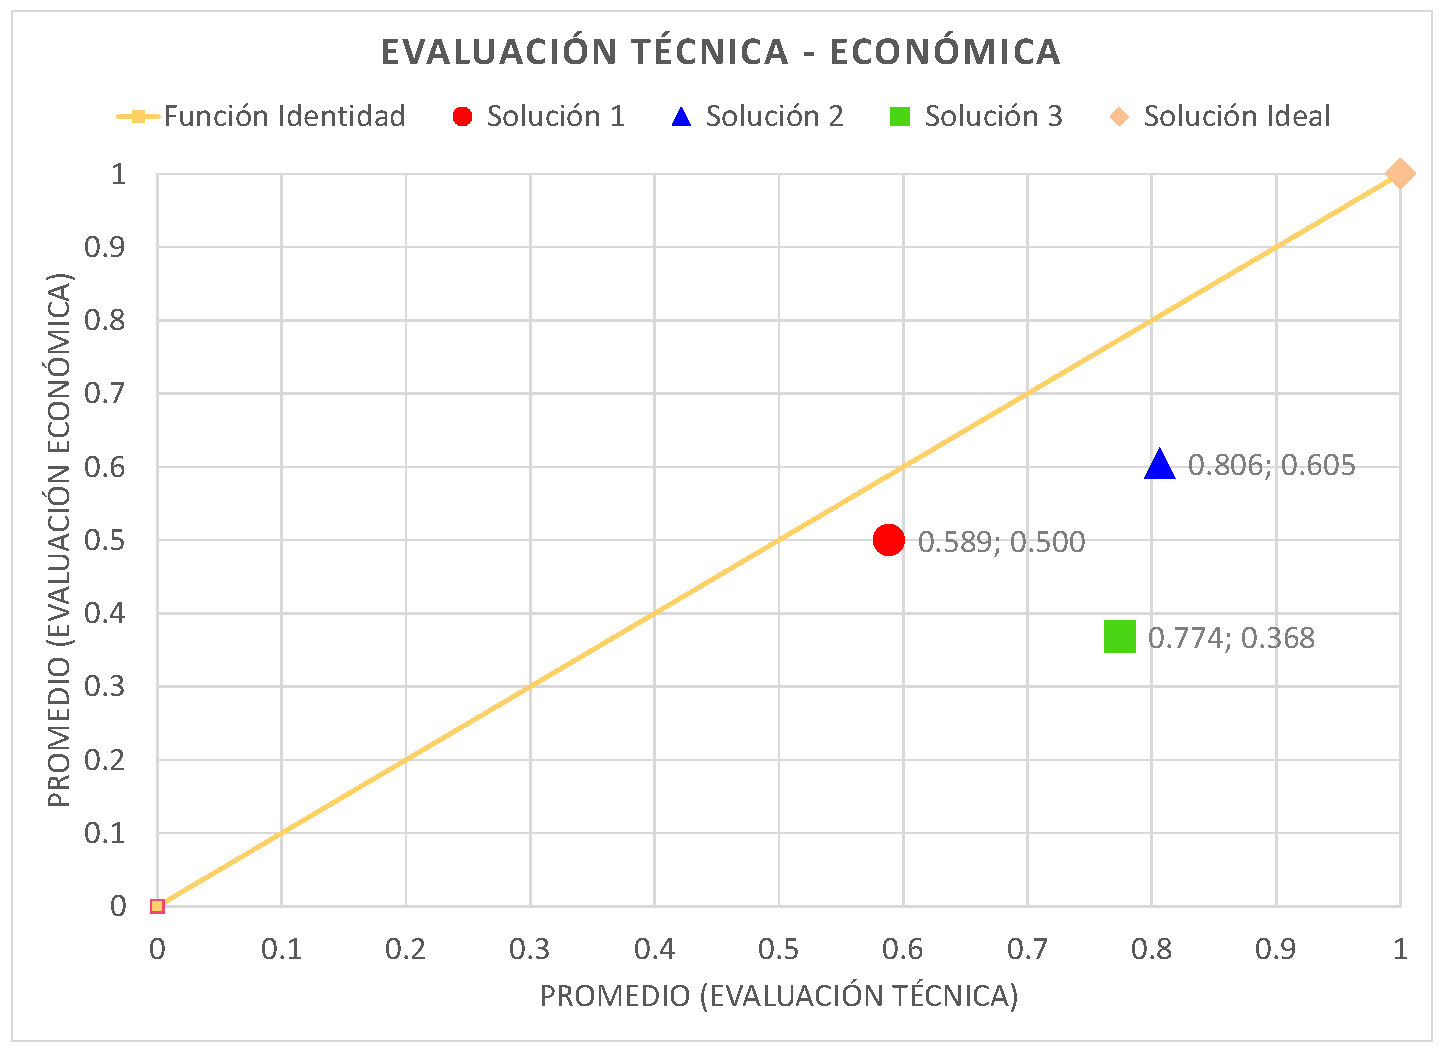
\includegraphics[width=0.8\textwidth]{img/EVALUACIONES.pdf}
	\caption[Gráfica de comparación técnico-económica de los conceptos de solución.]{Gráfica de comparación técnico-económica de los conceptos de solución. Fuente: Elaboración propia.}
	\label{fig:comp_tecnico_economica}
\end{figure}

\section{Diagrama de funcionamiento del concepto de solución óptimo}

\begin{figure}[H]
	\centering
	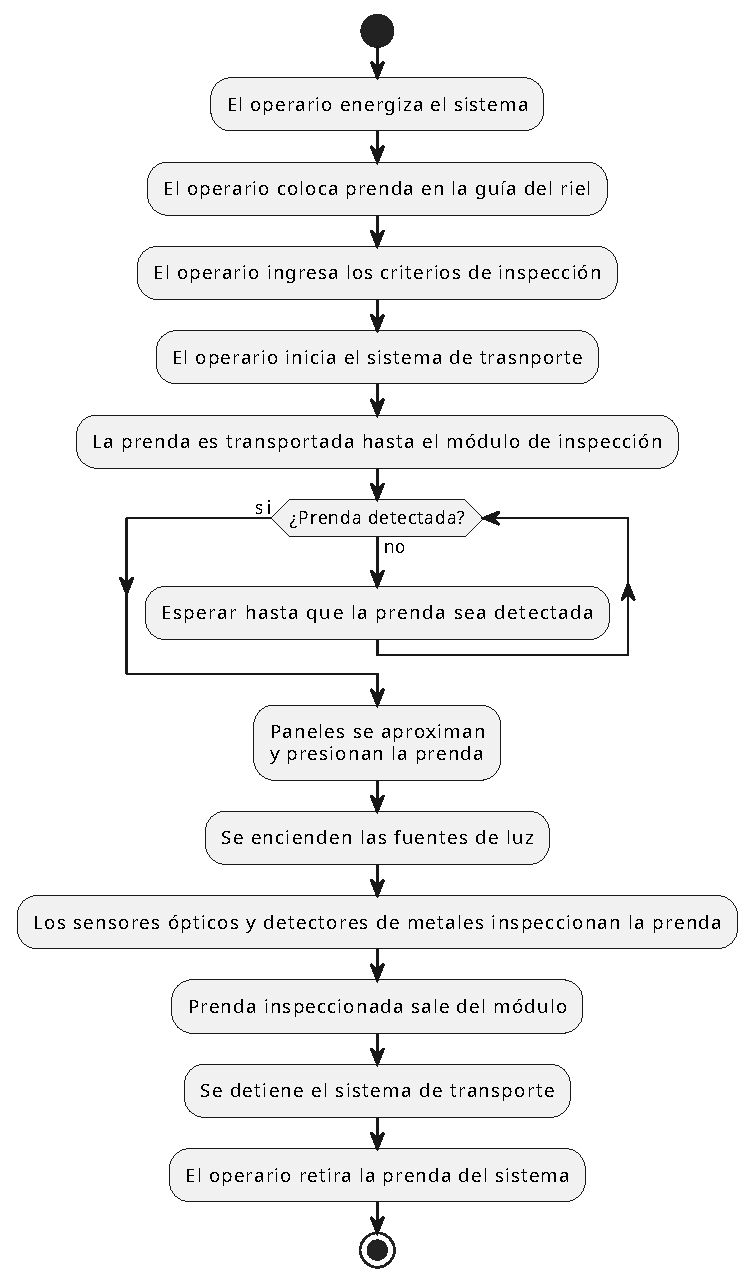
\includegraphics[width=0.8\textwidth]{img/diagrama_flujo.pdf}
	\caption[Diagrama de funcionamiento del sistema.]{Diagrama de funcionamiento del sistema. Fuente: Elaboración propia.}
	\label{fig:diagrama_flujo}
\end{figure}
